
%!TEX root = ../thesis.tex
%*******************************************************************************
%****************************** Third Chapter **********************************
%*******************************************************************************
\chapter{Simulation Framework of SBND}
\label{ChapterSim}

% **************************** Define Graphics Path **************************
\ifpdf
    \graphicspath{{Chapter5/Figs/Raster/}{Chapter5/Figs/PDF/}{Chapter5/Figs/}}
\else
    \graphicspath{{Chapter5/Figs/Vector/}{Chapter5/Figs/}}
\fi

%********************************** %Opening  **************************************

%Modern physics experiments and MC
Many modern particle physics experiments heavily rely on simulations to assess the physics capabilities of the detector, to develop physics analysis tools as well as to relate experimental data to an underlying theoretical model they attempt to probe.  
The most common simulation technique is Monte Carlo (MC), by random sampling from Probability Density Functions (PDFs).
PDFs can be modelled from theories or derived from experimental data or a combination of both.
%Simulation is beneficial for an experiment like SBND in the early stage of development where the detector is not yet operational to record data.
The search for Heavy Neutral Leptons (HNLs) at the Short-Baseline Near Detector (SBND) presented in this thesis employs simulated MC samples mimicking data.                                 
This enables an exploration of the detector physics capabilities in the regime of physics beyond the Standard Model (BSM).
%, given that the detector timing resolution can achieve nanosecond resolution.

The following chapter provides a description of the simulation framework of SBND to output simulated products representing real data.
The chapter begins with an overview of the framework in Section \ref{sec:overview_sim}.
Following that, Section \ref{sec:gen_mevprtl} includes details of the generator employed to generate HNLs, of which its development was contributed by the author.
The summary of the generators of SM neutrinos and cosmic muons is given in Section \ref{sec:gen_sm}.
Section \ref{sec:gen_response} covers the simulation of energy deposition as particles propagate through the detector and the detector response to the deposited energy.
Finally, the chapter is concluded in Section \ref{sec:sim_concluding_remarks} with some remarks.

%********************************** %First Section  **************************************
\section{Overview of the Simulation Framework}
\label{sec:overview_sim}

The software framework for simulation, reconstruction and analysis of SBND is provided by the LArSoft framework \cite{larsoft}. 
The framework was originally built for Liquid Argon Time Projection Chamber (LArTPC) neutrino experiments, allowing for detector-specific customisation. 
This enables easy sharing of software tools across many collaborations including ArgoNeuT, MicroBooNE, ICARUS, SBND and DUNE. 
For example, the generator used to simulate HNLs, presented in Section \ref{sec:gen_mevprtl} next, has been developed and shared across the SBND and ICARUS collaborations.

%Describe the overall workflow
The simulation workflow of SBND under LArSoft is depicted in Fig. \ref{fig:Sim_Workflow}.
The process begins with a generator to produce primary particles that enter the TPC, as shown by the purple box.
The primary particles can be final states of neutrino interactions, cosmic muons or BSM particles depending on the generator type.
The propagation of the primary particle inside and outside the TPC, and the resulting energy deposition is simulated using the Geant4 toolkit \cite{geant4}, as shown by the green boxes.
For interactions inside the detector, the charge and light yield are calculated from the energy deposition.
Ionisation electrons are propagated through the detector to the wire planes using the Wirecell toolkit \cite{wirecell}, as shown by the red boxes.
Scintillation photons are propagated to the photodetectors using a combination of a semi-analytical model and an optical library \cite{sbnd_pds_paper}, as shown by the blue boxes.
For interactions outside of the detector, only the energy depositions within Cosmic Ray Tagger (CRT) strips are converted into light yield, as shown by the orange box.
The detector response is then simulated for each detector subsystem.
By the end of this stage, the outputs from each detection subsystem ideally represent real data.

\begin{figure}[htbp!] 
\centering    
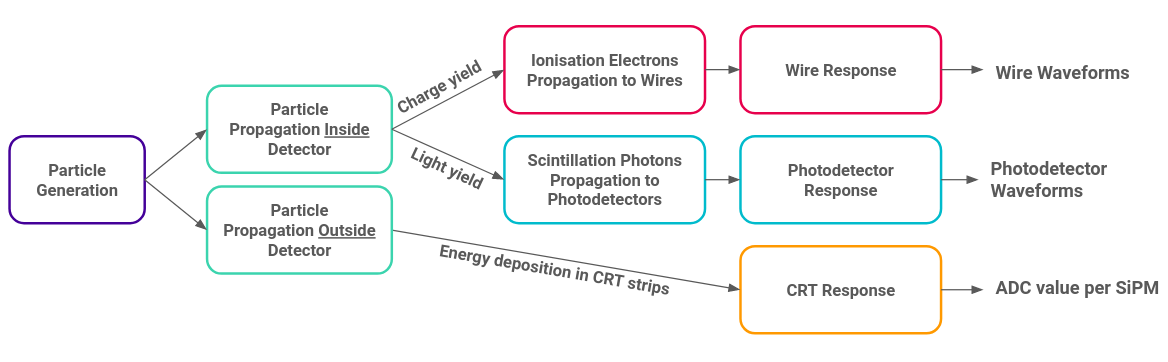
\includegraphics[width=1.0\textwidth]{Sim_Workflow}
\caption[Simulation Framework of SBND]{
Overview of the simulation framework of the SBND detector.
}
\label{fig:Sim_Workflow}
\end{figure}

\section{HNL Generator: MeVPrtl}
\label{sec:gen_mevprtl}

%MeVPrtl Workflow
BSM particles are generated using a generator called MeVPrtl, which was developed as a joint effort by collaborators from both ICARUS and SBND experiments.
There are several BSM models implemented in the MeVPrtl generator, including HNLs, Higgs portal scalars \cite{higgs_scalar} and heavy quantum chromodynamics axions \cite{qcd_axion}.
It is a modular generator, allowing for easy adaptations for different beam sources and detectors, as well as a direct interface with LArSoft.
The workflow of the MeVPrtl is broken down into four stages, as illustrated in Fig. \ref{fig:MeVPrtl_Workflow}.
The generator begins with taking an input of meson fluxes produced from a beam source.
It then simulates the meson decaying to a BSM particle.
The BSM particle is propagated to the detector and decays back into SM observables.

\begin{figure}[htbp!] 
\centering    
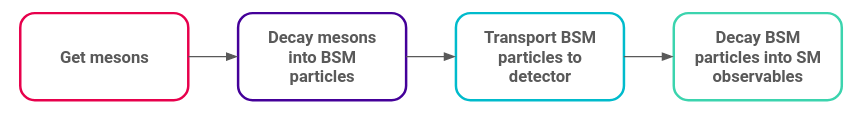
\includegraphics[width=1.0\textwidth]{MeVPrtl_Workflow}
\caption[MeVPrtl Generator Workflow]{
Overview of the workflow of the MeVPrtl generator.
}
\label{fig:MeVPrtl_Workflow}
\end{figure}

%Each stage validation
For generating HNLs coming from the Booster Neutrino Beam (BNB), the generator begins with sampling the $K^{+}$ fluxes of the BNB (See Fig. \ref{fig:BNB_Meson_Flux}, Section \ref{sec4BNB}).
Instead of decaying into SM neutrinos, the kaons decay into HNLs, with the branching ratio defined by Eq. \ref{eq:kaon_decay_hnl} (See Section \ref{sec2Production}).
The daughter HNL and lepton are simulated using the two-body decay at rest in the centre of mass frame of the parent kaon and then boosted to the parent's lab frame by Lorentz boost.
Due to HNLs having relatively high mass, the boost results in HNLs having less transverse momentum than the SM neutrinos, travelling preferably to the parent kaon direction.
The boost can also flip the directions of HNLs that are emitted backwards, mostly originating from low energy kaons \cite{DavidePhD}.

HNLs are then propagated to the detector by the ray tracing method, which picks a direction forcing HNLs to intersect SBND, defined as the TPC volume.  
%The probability of enforcing the detector intersection is also computed.
The acceptance angle of HNLs to hit the detector is very beam-collimated at $< \sim 5^\circ$ with respect to the beam direction.
This implies that only very forward-going HNLs are most likely to intersect the detector.

%Example angular distributions in the lab frame of parent kaons and HNLs that arrive at the SBND detector are shown in Fig. \ref{fig:kaon_hnl_angle2beam}.
%Fig. \ref{fig:kaon_angle2beam} shows the angle to the beam direction of 7 different kaon parents having energies peaking at approximately $0.5\sim1$ GeV, each of a different colour dashed line.
%The resulting HNL of mass 240 MeV from each kaon is shown in Fig. \ref{fig:hnl_angle2beam}, in the same colour dashed line as the parent kaon.
%Here, it can be seen that the angles to the beam direction of HNLs are very small as all the lines overlap within $ < 5^\circ$.
%
%\begin{figure}[htbp!]
%        \centering
%        \begin{subfigure}[b]{0.495\textwidth}
%            \centering
%            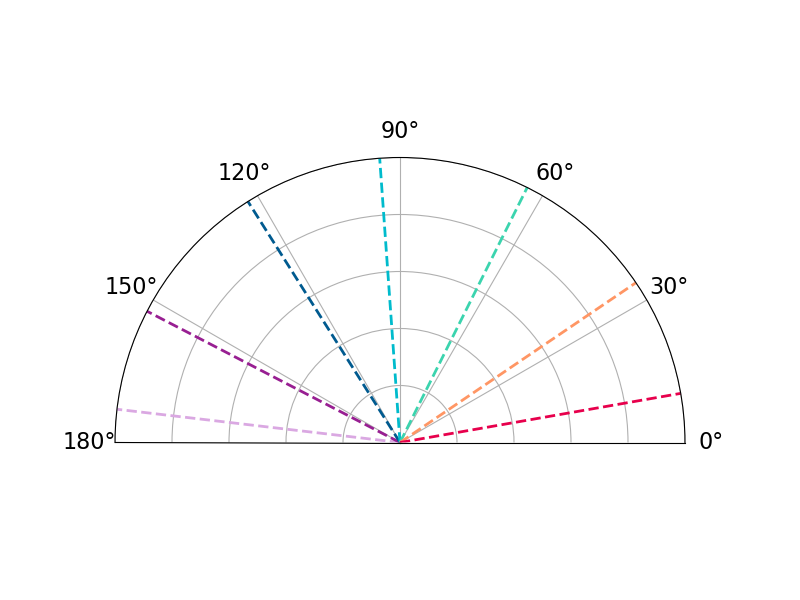
\includegraphics[width=\textwidth]{kaon_angle}
%            \caption{Kaons}%
%            \label{fig:kaon_angle2beam}
%        \end{subfigure}
%        \hfill
%        \begin{subfigure}[b]{0.495\textwidth}  
%            \centering 
%            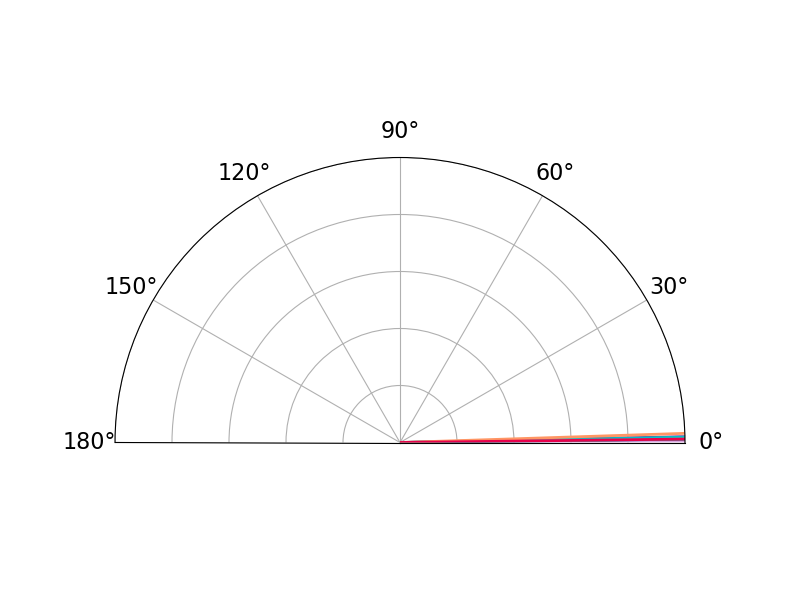
\includegraphics[width=\textwidth]{hnl_angle}
%            \caption{HNLs}%
%            \label{fig:hnl_angle2beam}
%        \end{subfigure}
%        \caption[Angle To The Beam Direction of Kaons and Resulting HNLs Polar Plots]{
%	Polar plots showing the angle to the beam direction of 7 different parent kaons (left) and of the resulting HNLs that arrive at the detector (right).
%	}
%        \label{fig:kaon_hnl_angle2beam}
%\end{figure}

The simulated total energy spectra of HNLs arriving at the SBND detector are depicted in Fig. \ref{fig:HNL_Energy_Spectrum} for the mass range between 140 and 260 MeV.
The spectra plotted here, and all subsequent kinematics plots in this section, are labelled \textit{true}, indicating they are at the truth level and not yet passed through detector simulation and reconstruction.
The spectra are normalised to the same coupling $|U_{\mu4}|^{2} = 1 \times 10^{-7}$ and an exposure of $1 \times 10^{21}$ Protons On Target (POT) projected for 3 years of data taking.
At the same coupling, the expected HNL rate decreases with lower mass since the branching ratio of $N \rightarrow \nu\pi^0$ decreases with lower mass (See Fig. \ref{fig:branchingRatio}, Section \ref{sec2Decay}).
Additionally, given that the $K^{+}$ total energy spectrum peaks at 0.5 GeV and decreases at higher energy (See Fig. \ref{fig:BNB_Meson_Flux}, Section \ref{sec4BNB}), the HNL spectra also concentrate at $<0.5$ GeV, and substantially decrease at higher energy. 
A peak near zero can also be seen in all energy spectra across the mass range, corresponding to HNLs resulting from Kaon Decay At Rest (KDAR).
Finally, the Kinetic Energy (KE) of HNLs is expected to decrease with higher mass.
This is due to HNLs coming from a kaon decay and therefore, the lighter the HNL mass, the more KE is available.

\begin{figure}[hb!] 
\centering    
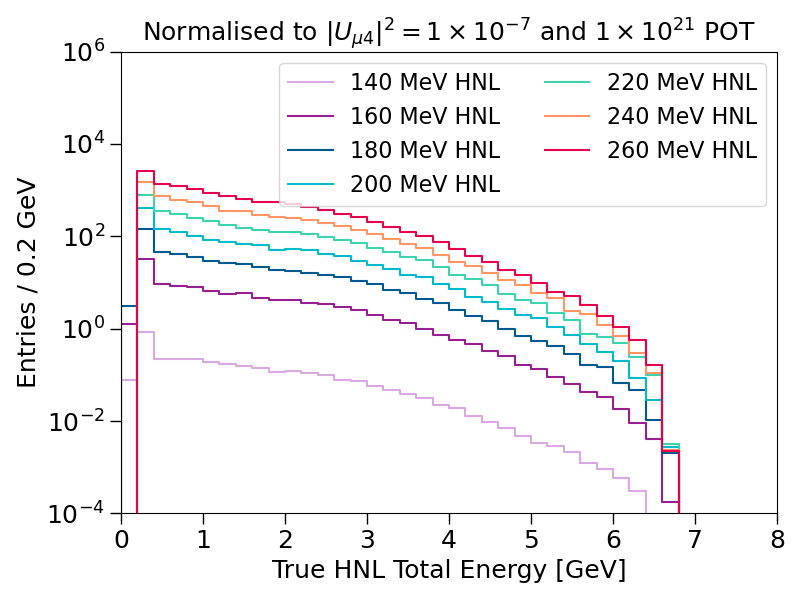
\includegraphics[width=0.65\textwidth]{HNL_Energy_Spectrum}
\caption[Simulated Energy Spectra of HNLs Decaying Inside SBND]{
Simulated energy spectra of HNLs decaying inside SBND.
}
\label{fig:HNL_Energy_Spectrum}
\end{figure}

HNLs are then simulated to decay back into the SM observables inside the TPC volume.
For the $\nu\pi^{0}$ final state, the width of the decay is defined by Eq. \ref{eq:pi0} (See Section \ref{sec2Decay}).
The kinematics of the decay products are simulated for HNLs isotropically decaying in the rest frame and then boosted to the lab frame by Lorentz boost.
%Since the parent HNL is very forward-going, the daughter $\pi^0$ is also forward-going, with momenta dependence on the mass of the parent HNL. 

Fig \ref{fig:pi0_distribution} shows the simulated true momenta and angle to the beam distributions of the $\pi^0$.
The plots are area-normalised for direct comparison across the HNL mass of 140-260 MeV. 
The peak in the momenta distribution at low GeV and the peak in the angular distribution at high angle are from the $\pi^0$ resulting from low energetic HNLs from KDAR.
Moreover, the momenta distribution of the $\pi^0$ decreases with increasing HNL masses.
This is due to the decreased boosting of HNLs at higher masses having less KE.
%since heavier HNLs are less energetic and therefore, less energy is available for the $\pi^0$.
As a result, the angle to the beam direction of the $\pi^0$ also widens with heavier HNLs.
However, at the heaviest HNL mass of 260 MeV considered in this work, the $\pi^0$ is still very beam-collimated since its angular distribution concentrates in the region $< 20^\circ$. 
Therefore, di-photon showers from the HNL-originated $\pi^0$ are expected to be more forward-going than those originating from SM neutrinos.

\begin{figure}[ht!]
%\vspace{0.5cm}
        \centering
        \begin{subfigure}[b]{0.495\textwidth}
            \centering
            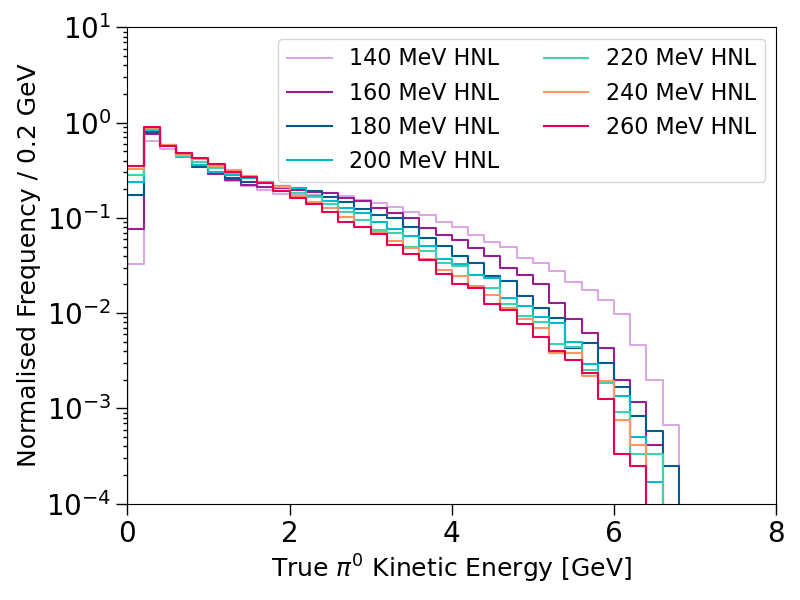
\includegraphics[width=\textwidth]{pi0_energy}
            \caption{Momentum}%
            %\label{fig:kaon_angle2beam}
        \end{subfigure}
        \hfill
        \begin{subfigure}[b]{0.495\textwidth}  
            \centering 
            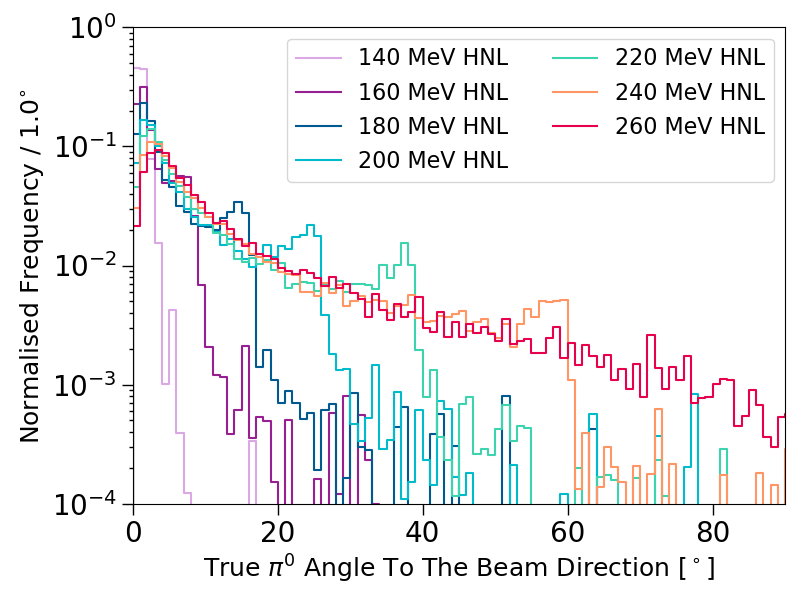
\includegraphics[width=\textwidth]{pi0_angle2Beam}
            \caption{Angle to the beam direction}%
            %\label{fig:hnl_angle2beam}
        \end{subfigure}
        \caption[Simulated Kinematics Distributions of Neutral Pions from HNLs]{Simulated kinematics distributions of $\pi^0$ from HNLs decaying inside SBND.}
        \label{fig:pi0_distribution}
\end{figure}

The timing delay of HNLs compared to SM neutrinos due to HNLs being more massive can be exploited in the search for HNLs at SBND. 
The components that make up the time of flight for an HNL or a SM neutrino produced from the BNB and propagating to the SBND detector are illustrated in Fig. \ref{fig:tof_beam_to_detector}.
The first component is the spill time of the protons from the Booster synchrotron, $t_{\mathrm{spill}}$, as shown by the red arrow.
The structure of $t_{\mathrm{spill}}$ is the beam bucket structure made up of 81 Gaussian buckets with a width of 1.308 ns and a spacing of 19 ns (See Section \ref{sec4BNB}).

The second component is the time of the secondary mesons, $t_{\mathrm{meson}}$, as shown by the blue arrow.
This is the period from when the mesons are produced until they decay into HNLs or SM neutrinos.
This time accounts for the duration that the mesons travel down the decay pipe, and might interact, re-scatter or decay into other mesons.
In the case of HNLs, $t_{\mathrm{meson}}$ is primarily the time of flight of the $K^+$ before decaying into an HNL.
On the other hand, SM neutrinos come from a variety of parent mesons $t_{\mathrm{meson}}$. % (See Fig. \ref{fig:BNB_neutrino_flux}).
In both cases, $t_{\mathrm{meson}}$ introduces some smearing to the nanosecond-bucket structure of $t_{\mathrm{spill}}$.

The last component is the time of flight of the SM neutrino or the HNL from the production to the interaction location inside the SBND detector.
In the case of SM neutrinos, since they are nearly massless, their velocity can be approximated as the speed of light. 
The time of flight of SM neutrinos is:  
\begin{equation}
	t_{\nu} = \frac{d_{\nu}}{c},
\end{equation}
where $d_{\nu}$ is the distance of a neutrino from the production to the interaction location inside the detector.
Meanwhile, HNLs are massive and travel at a velocity $v_N < c$.
The time of flight of HNLs is:
\begin{equation}
	t_{N} = \frac{d_{N}}{v_N},
\end{equation}
where $d_N$ is the distance of a HNL from the production to the decay location inside the detector.
Additionally, since the KE of HNL decreases with its mass, the heavier it is, the slower its velocity.

\begin{figure}[hb!] 
\vspace{0.5cm}
\centering    
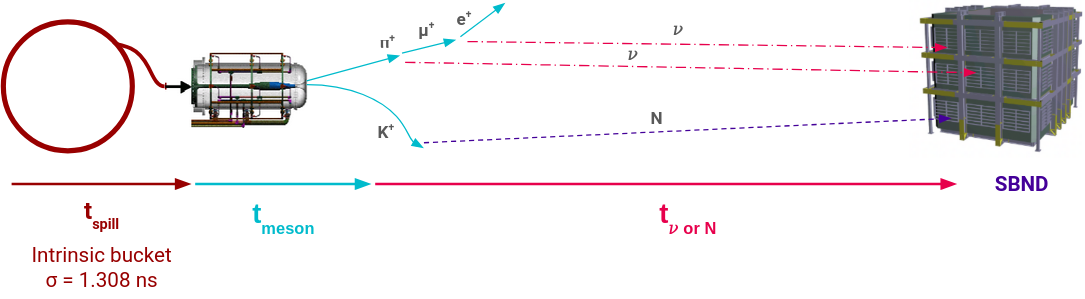
\includegraphics[width=1.0\textwidth]{tof_beam_to_detector}
\caption[Time of Flight of Particles from the BNB to SBND Diagram]{
The time of flight of a particle from the production to the detection location in the SBND detector.
}
\label{fig:tof_beam_to_detector}
\end{figure}

\begin{figure}[b!] 
\centering    
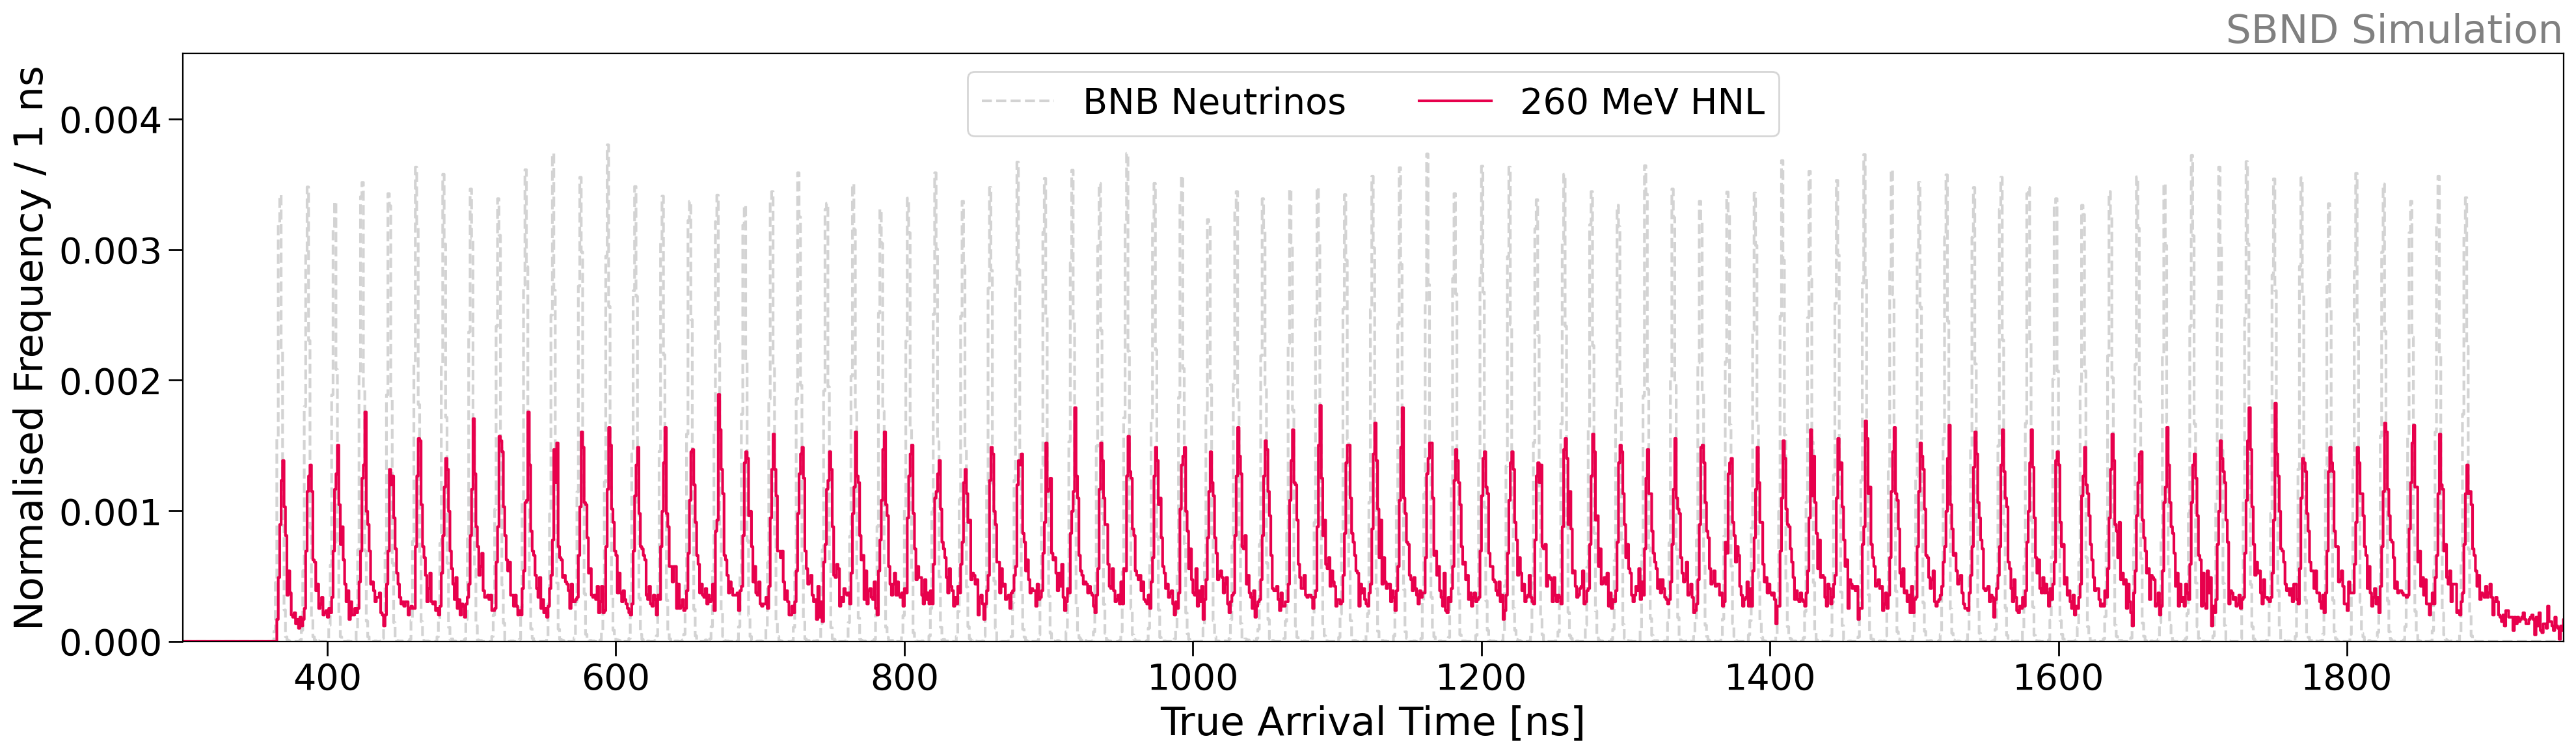
\includegraphics[width=1.0\textwidth]{full_beam}
\caption[Arrival Time of SM Neutrinos and HNLs at the Front Face of SBND]{
True arrival time distribution at the front face of the SBND detector for SM neutrinos and HNLs. 
}
\label{fig:full_beam}
\end{figure}

The advantage of the MeVPrtl generator is the consistency of simulating the time of flight of HNLs compared to the GENIE generator \cite{genie} for simulating SM neutrinos.
Fig. \ref{fig:full_beam} shows the simulated true arrival time of SM neutrinos, in the dashed grey line, and 260 MeV HNLs, in the solid red line, at the front face of the SBND detector, recovering the beam bucket structure of the BNB.
The plot is area-normalised to enable a direct comparison between the two particles. 
Since SM neutrinos travel nearly at the speed of light, less smearing is introduced and the arrival time distribution shows sharp Gaussian peaks.
On the other hand, HNLs travel at a slower velocity, resulting in excesses on either sides of the Gaussian peaks.

For clarity, shown in Fig. \ref{fig:beam_modulus} is the result of 81 Gaussian peaks overlaid into a single peak by applying a modulus of 19 ns.
The arrival time distribution of HNLs is distinctively different from that of SM neutrinos, where excesses on either side of the Gaussian peak of SM neutrinos can be seen.
It is important to note that excesses before the neutrino peak is due to the HNL tail of one bucket leaking into the next one.
Between the mass of 140 to 260 MeV, the HNL excesses however do not increase significantly with mass.

\begin{figure}[ht!] 
\vspace{0.5cm}
\centering    
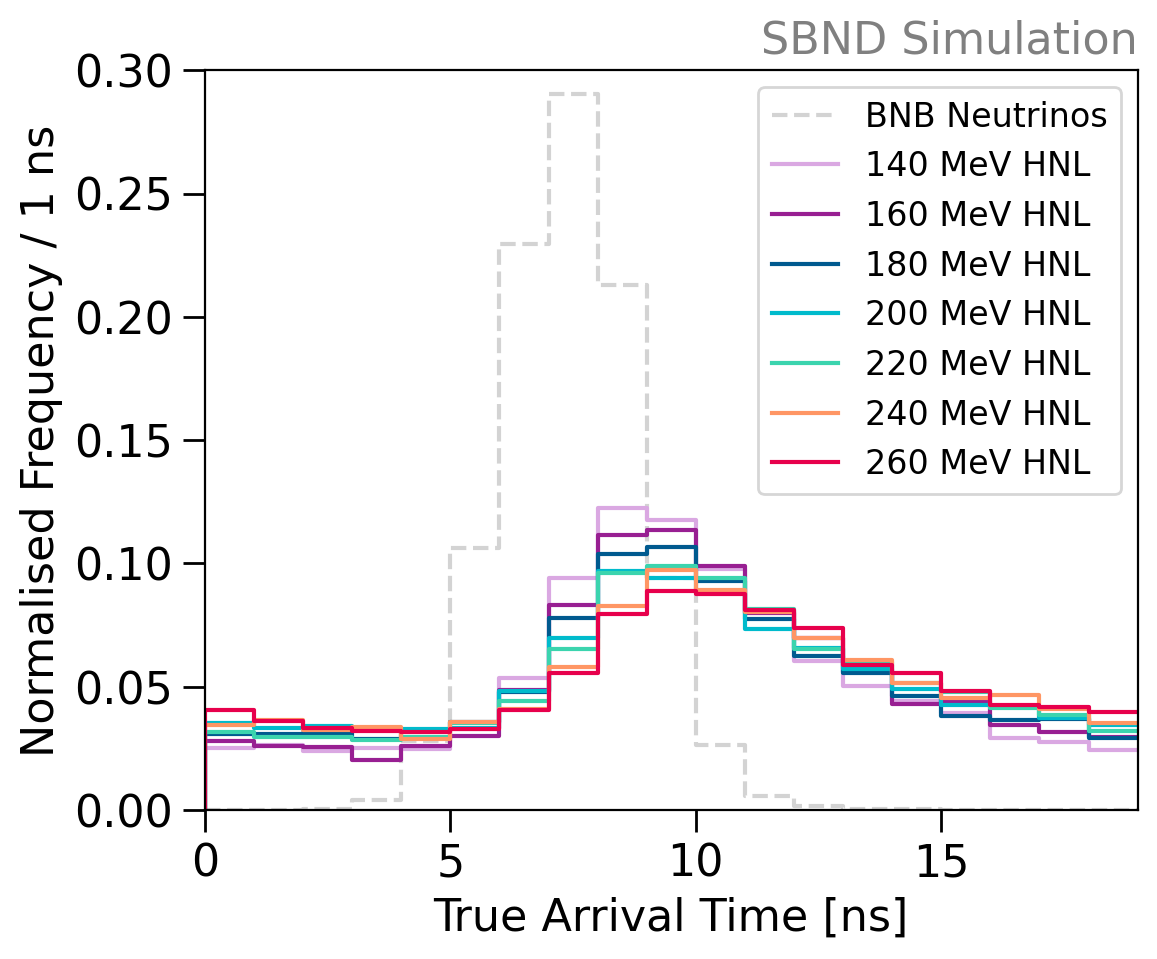
\includegraphics[width=0.495\textwidth]{beam_modulus}
\caption[Modulus of the Arrival Time Distibutions of SM Neutrinos and HNLs]{
True arrival time distribution for SM neutrinos and HNLs after applying a modulus of 19 ns . 
}
\label{fig:beam_modulus}
\end{figure}

\section{Standard Model Generators}
\label{sec:gen_sm}

For generating backgrounds from SM neutrinos and cosmic muons, the two generators are GENIE \cite{genie} and CORSIKA \cite{corsika} respectively.
Each generator is discussed in Section \ref{sec:gen_genie} and Section \ref{sec:gen_corsika}.

\subsection{Neutrino Generator: GENIE}
\label{sec:gen_genie}

%Overview of GENIE
SM neutrino interactions are generated by the GENIE generator \cite{genie}, which provides a selection of theoretical and empirical models for different physical processes.
These models can be combined into a \textit{tune}, which is a set of optimised parameters used in the simulation for a better agreement between model and data.
The GENIE tunes are made using an extensive dataset of electron, neutrino and hadron scattering experiments.
SBND is using a tune that was developed to serve as a baseline model for the Short-Baseline Neutrino program and DUNE oscillation analysis, named \texttt{AR20i\_00\_000}.
The tune was developed using the base configuration \texttt{G18\_10a\_02\_11b}, of which the details can be found in Ref. \cite{genie_tune}.
Ongoing developments of the tune is documented in Ref. \cite{genie_tune_github}.  

%What kind of tune are being used
GENIE first selects a nuclear model that describes the momenta and potential energy of the nucleon to model nuclear effects.
Then, neutrino fluxes and integrated cross section models are used to compute the probability that a neutrino interaction occurs.
Differential cross section models are used next to determine the type of neutrino interaction and the kinematic range.
Neutrino interaction types include quasi-elastic, resonant, coherent, deep inelastic and $\nu$-e elastic scatterings.
In addition, a neutrino interacting with an argon nucleus can produce hadrons within the nucleus.
The hadrons propagate through the nucleus, interacting via different modes such as charge exchange, elastic scattering, absorption and pion production.
Consequently, hadron-nucleus interactions modify the final state particles and their kinematics.
Thus, hadron transport interaction models are crucially important for predicting the final observables of neutrino interactions.

%model used for resonant production, coherent pion production
Relevant to the search for HNLs with a neutral pion in the final state, the main SM neutrino interaction backgrounds are the neutral current resonant and coherent pion production.
From the tune \texttt{AR20i\_00\_000}, the model used for these two interaction modes is called Berger-Seghal \cite{genie_tune, piontune}.
For resonant pion production, the model computes the cross section of baryon resonances, where the baryons are simulated to decay into pions isotropically.
For coherent pion production, the model computes the pion-nucleus cross section, requiring a small momentum transfer to the target nucleus.
GENIE does not apply the formation time to pions from these two modes, since the former results from baryon decays and the latter does not interact with the nucleus.
The resulting pions are then simulated to propagate outside the nucleus, with a propagation time $\mathcal{O}$(1-10~ys).
This demonstrates the emission time of pions from SM neutrino interaction is almost instantaneously, significantly smaller than the late arrival of HNLS to the detector.

GENIE also provides uncertainties for a chosen model that can input to a reweighting scheme for uncertainty assessment.
Due to the scarcity of neutrino interaction data, particularly for $\nu$-Ar interactions, uncertainties of cross section modelling tend to be very large. 
Uncertainties of SM neutrino cross section is discussed in Section \ref{sec:bkg_error}.

At SBND, GENIE simulates neutrino interactions occurring both inside and outside of the detector volume, with a boundary defined in Fig. \ref{fig:Rockbox_Volume}.  
All interactions occurring inside the detector volume are kept, as shown by the dark blue box.
Outside of the detector, a buffer volume is defined as 5 m surrounding the detector volume, as shown by the light blue box.                       
An additional Rockbox volume is defined by extending the buffer volume backwards in the beam direction ($z$-axis) up to 15 m in front of the buffer volume, as shown by the orange box.
%Both these volumes are referred to together as the \textit{Rockbox} volume in this thesis.
Neutrino interactions within this volume are kept because their products can potentially deposit energy inside the detector.
These interactions are referred to as \textit{dirt} neutrinos and constitute a significant background to the HNL search.
The background rejection of dirt neutrinos is covered in Chapter \ref{ChapterSelect}.

\begin{figure}[hb!] 
\centering    
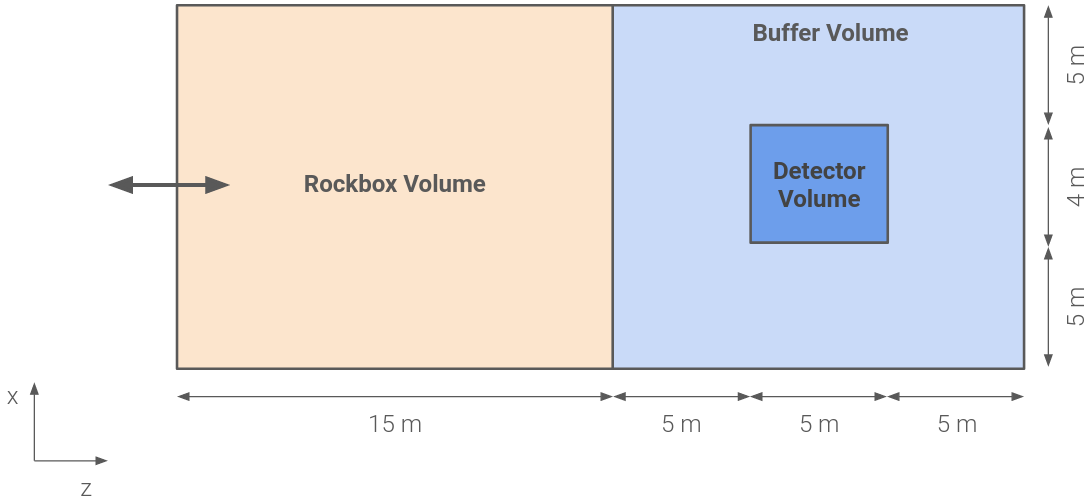
\includegraphics[width=0.85\textwidth]{Rockbox_Volume}
\caption[Volume Boundary of the GENIE Generator]{
Volume boundary defined by the GENIE generator to simulate neutrino interactions occurring inside and outside of the detector volume. 
}
\label{fig:Rockbox_Volume}
\end{figure}


\subsection{Cosmic Generator: CORSIKA}
\label{sec:gen_corsika}

Cosmic interactions are simulated using the CORSIKA generator \cite{corsika}.
The generation begins with producing high energy primary particles incident in the Earth's atmosphere.
The simulation adopts the same approach as the MicroBooNE experiment where primary particles are modelled as cosmic protons, motivated by a better data agreement as seen by MicroBooNE \cite{corsika_uboone}.
The primaries are then propagated through the atmosphere, interacting with the air to produce secondary hardons that decay into long-lived particles reaching the Earth's surface.
Within the SBND simulation geometry, this surface is specified to be just above the roof of the detector building.
The surviving particles are then propagated to the SBND detector.

%Why cosmic simulation is important
From a triggering perspective, there are two types of cosmic muons as follows:
\begin{coloritemize}
        \item\textbf{In-time} cosmic muons cross the detector at the same time as SM neutrinos being present inside the detector, such that the muons are \textit{inside} the beam spill window. The cosmic muons produce enough light to induce a beam trigger.                            
        \item\textbf{Out-of-time} cosmic muons occur regardless of the trigger conditions. The muons cross the detector \textit{outside} the beam spill window but within the readout window.  
\end{coloritemize}
However, at the time of writing, triggering simulation is currently a work in progress at SBND and is not simulated in the workflow. 
Only the timing requirement is simulated to keep only cosmic muons occurring within the readout window.
The simulation currently does not accurately reflect the cosmic rate once factoring triggering conditions and therefore, a comparison to data is necessary. 

Being a surface-level detector, it is vitally important to understand the cosmic background at SBND due to the high cosmic exposure.
Once SBND is operational, a particularly useful measurement is the rate of cosmic muons that cause a beam trigger, however, in the absence of the beam.
This is equivalent to measuring the rate of cosmic muons that produce sufficient energy inside the detector to mimic SM neutrino interactions.
This measurement allows for validation against the CORSIKA generator.
Moreover, it also provides an expected cosmic rate given a triggering condition, which can be added to the simulation framework to better constrain the cosmic background.                
%sampling of the cosmic topology and kinematic distribution. 

\section{Particle Propagation and Detector Response Simulation}
\label{sec:gen_response}

Simulated particles are propagated through the detector and deposit energy, producing ionisation electrons and scintillation photons.
Detector responses to the ionisation electrons and scintillation photons are subsequently simulated, mimicking data. 
Section \ref{sec:gen_g4} first covers the simulation of particle propagation and energy deposition.
Following that, Section \ref{sec:wire_response}, \ref{sec:pds_response} and \ref{sec:crt_response} provides a description of the simulation of the Time Projection Chamber (TPC), Photon Detection System (PDS) and CRT response. 

\subsection{Particle Propagation Simulation}
\label{sec:gen_g4}

Once a particle is simulated inside the detector, it is propagated through the detector using the Geant4 toolkit \cite{geant4}.
Geant4 propagates the particle by each step $dx$, where the step length is randomised and capped at 0.3 mm (one order of magnitude less than the wire pitch).
At each step, physics processes are simulated, such as energy deposition, interaction, decay and so on.
The step propagation also accounts for the electric field distortion caused by the space charge effect due to high exposure to cosmic muons.
%For example of the $\nu\pi^0$ final state of HNLs, the $\nu$ escapes the detector without interacting while the $\pi^0$ is simulated to decay into a di-photon shower by Geant4.
%Then, Geant4 simulates the energy deposition of the resulting di-photon shower.

The main physics process for energy deposition in the detector is ionisation by charged particles.
Similarly to the theory detailed in Section \ref{sec3:creation}, the Geant4 toolkit simulates the ionisation process following the Bethe-Bloch formalism tuned to data \cite{geant4_ions}.
The number of ionisation electrons and scintillation photons from the deposited energy is computed using the modified Box recombination model with ArgoNeuT parameters \cite{argoneut_recomb}, and the charge-light anti-correlation from Eq. \ref{eq:Q} and \ref{eq:L}. 
Details of the ionisation simulation are further discussed in Section \ref{sec7:delta}.
The result from the Geant4 toolkit is a complete set of charge and light yields along the primary particle trajectories through the detector and the daughter particles produced from the primary.

\subsection{Wire Response Simulation}
\label{sec:wire_response}

Ionisation electrons are simulated to drift towards the wire planes using the WireCell toolkit \cite{wirecell}.
The simulation transports the electrons and introduces smearing due to detector effects for transporting electrons through liquid argon under an electric field.
This includes charge attenuation due to impurities, longitudinal and transverse diffusion and finally, space charge effect (See Section \ref{sec:edrift}).

Once drifting electrons arrive at the wire planes, a convolution of the field response and the electronic response is performed.
The field response describes the current induced on wires due to ionisation electrons drifting past the induction planes.
The electronic response describes the amplification and shaping of each wire's induced current by pre-amplifiers.
The response functions are in two dimensions, time versus wire, to account for the long range charge induction effect on wire signal shapes.
A digitisation step is applied to produce an ADC-level, time-domain waveform for each wire channel.
The waveform is parameterised by the ADC resolution, voltage range and baseline specification of the wire readouts.
Finally, inherent electronic noise is added to the waveform to better match to observed data.
MC waveforms at this stage should represent real data waveforms.

\subsection{Photon Detection System Response Simulation}
\label{sec:pds_response}

Scintillation photons are simulated to propagate to optical detectors, accounting for transport effects such as Rayleigh scattering and boundary effects (See Section \ref{sec:photonprop}).
Technical details of the light simulation can be found in Ref. \cite{sbnd_pds_paper}.
Instead of fully performing ray tracing of photons that can be computing intensive, the simulation uses a combination of a semi-analytical model and an optical library model to effectively estimate light detection probability. 
The choice of which model to use depends on the location of the photon production.
The semi-analytical model, as described in Ref. \cite{pds_sim}, is used for those produced inside the TPC volume.
The optical library model, readily available in LArSoft, is used for those that originate outside of this volume.

The semi-analytical model calculates on-the-flight the geometrical aperture for each optical detector to a scintillation location, given that the emission of scintillation photons is isotropic.
%The model also extends to both direct visible photons and also reflected VUV photons. 
Corrections for photon transport effects are applied to the number of photons detected by an optical detector.
However, the semi-analytical method is limited by the geometrical information and does not include scintillation outside the TPC volume, for example, cosmic muons crossing behind an optical detector can produce non-negligible photons.
Since PMTs are the primary subsystem for triggering, it is vital to consider this second-order contribution of photons for triggering studies.
The optical library stores information of the fraction of incident photons for each optical detector for a given scintillation location, which can be looked up for any detector-location pairs during 
simulation. 

For each type of optical detector, PMTs and X-ARAPUCAs, a respective photon detection efficiency is applied to the number of detected photons.
Signal amplification and digitisation are simulated, converting photons into an output signal known as a single electron response.
Then, signal shaping such as overshoot and undershoot due to the AC circuit of the optical detectors are applied.
Finally, random fluctuation in the signal integral and non-linearity response at high light intensities are applied to better mimic data.
The output is MC optical waveforms for each detector type, mimicking data. 

\subsection{Cosmic Ray Tagger Response Simulation}
\label{sec:crt_response}

The energy deposition outside of the cryostat from the Geant4 simulation stage is considered if it is within CRT strips.
It is converted into photons within a strip and propagated down optical fibres towards the SiPMs for detection.
The collection efficiency per SiPM is accounted for by dividing the light yield between the fibres on either side of the strip, based on the lateral position of the energy deposition within the strip.
Propagation effects and signal attenuation are also simulated.
Finally, the electronic response is simulated for the CRT readout, by assessing if a pair of SiPMs within a strip goes above a threshold within a coincidence window.
To better mimic the readout electronics of CRTs that process 32 SiPMs at a time, MC outputs of CRTs are in a group of 32 ADC values, where each value corresponds to a SiPM.

\section{Concluding Remarks}
\label{sec:sim_concluding_remarks}

The simulation framework of SBND is an end-to-end process, starting from the particle production, to its energy deposition and subsequently, the detector response to the energy deposition.
MC outputs of the simulation mimic data, enabling studies to understand and improve the detector performance as well as to compare against theoretical models.
For example, Chapter \ref{ChapterReco} next provides a description of the reconstruction framework at SBND, of which many algorithms have been developed using MC samples.
Furthermore, calibration studies presented in Chapter \ref{ChapterCalib} were carried out using MC samples of protons and muons to better understand the particle-dependent energy deposition.
Finally, the search for HNLs presented in the two final Chapters \ref{ChapterSelect} and \ref{ChapterResult} was also performed using MC samples to explore the physics capability of SBND.
